\chapter{Preliminary Results and Discussion}
\label{chap:results}

\section{Status of the Analysis}
This chapter reports the workbook snapshot retrieved on 22 September 2026~\cite{srooranalysis}. It is a provisional description of the available outputs, not an approved final analysis. The workbook marks its calculation run as complete, but explicitly marks the data as unsafe to interpret because six blocking data-quality errors remain. It also lists 130 unreviewed, uncounted responses.

The distinction affects every result below. A stored mean and confidence interval can be arithmetically correct while relying on records whose scoring or inclusion still needs review. The visible blocking errors include duplicate eligible questionnaire records. Legacy presence scoring, unresolved responses, mixed list versions, and unavailable order diagnostics create further limitations.

For this draft, the reported recall means, paired differences, $t$ statistics, and $d_z$ values were checked against the workbook's included trial-level accuracy values. They agree within rounding tolerance. This verifies the transcription and arithmetic of the snapshot, not the correctness of all source decisions. A pseudonymous local snapshot and a small verification script accompany the thesis source.

\section{Available Observations}
Table~\ref{tab:coverage} reports complete-pair counts for the main outcomes. The number of participants differs by measure. A missing outcome was not replaced with zero, and the maximum number of available recall pairs was not reused as the sample size for every questionnaire.

\begin{table}[htbp]
\centering
\caption{Complete pairs available in the provisional workbook snapshot.}
\label{tab:coverage}
\begin{tabular}{lr}
\toprule
Outcome & Complete pairs \\
\midrule
Immediate recall accuracy & 18 \\
Nominal 24-hour recall accuracy & 16 \\
Nominal one-week recall accuracy & 14 \\
Immediate recall duration & 14 \\
IMI subscales & 17 \\
SUS presence & 14 \\
Cognitive-load subscales & 18 \\
Legacy IPQ comparison & 0 \\
Session-order diagnostic & 0 \\
\bottomrule
\end{tabular}
\end{table}

The included recall records comprise 36 immediate trials, 32 nominal 24-hour trials, and 28 nominal one-week trials. The 36 immediate records include eight 20-target Condition List trials, twelve 25-target Memory List trials, and sixteen 25-target Hard Memory List trials. Thus, the immediate comparison pools more than one materials version.

These counts do not establish a final recruitment flow. Some sessions may belong to pilot development, and the participant registry still requires review. The final report needs a separate account of recruitment, exclusions, main-study eligibility, and missing outcomes.

\section{Recall Accuracy}
Table~\ref{tab:recallmeans} gives the condition means and standard deviations for accuracy. Each row uses the same complete paired subset for its two condition means. Different timepoints can involve different subsets.

\begin{table}[htbp]
\centering
\small
\caption{Provisional recall accuracy as a percentage of the trial's target list. SD denotes sample standard deviation.}
\label{tab:recallmeans}
\begin{tabular}{lrrr}
\toprule
Timepoint & $n$ & Generic mean (SD) & Personalised mean (SD) \\
\midrule
Immediate & 18 & 72.39 (26.21) & 78.67 (24.46) \\
24 hours & 16 & 59.63 (29.58) & 66.13 (29.71) \\
One week & 14 & 52.07 (32.57) & 57.43 (30.89) \\
\bottomrule
\end{tabular}
\end{table}

Immediate accuracy is numerically higher in the personalised condition by 6.28 percentage points. The workbook's paired estimate has a 95\% confidence interval from $-2.51$ to 15.06 percentage points, $t(17)=1.508$, $p=.150$, and $d_z=0.355$. Eight participants have higher personalised scores, seven have higher generic scores, and three have equal scores. The median paired difference is zero.

The mean difference therefore does not describe a uniform benefit across participants. It also does not establish equivalence: the interval includes both a negative difference and a potentially meaningful positive difference. Even if the underlying records were fully reconciled, the uncertainty would remain important. In the present snapshot, the data-quality block provides an additional reason to withhold a final conclusion.

At the nominal 24-hour follow-up, the paired difference is 6.50 percentage points, with a 95\% interval from $-4.33$ to 17.33. At one week, it is 5.36 percentage points, with an interval from $-1.26$ to 11.97. Table~\ref{tab:recalltests} reports the corresponding stored statistics.

\begin{table}[htbp]
\centering
\small
\caption{Provisional paired recall comparisons. Differences and confidence intervals are in percentage points, personalised minus generic. All $p$ values shown are unadjusted.}
\label{tab:recalltests}
\begin{tabular}{lrrrrr}
\toprule
Timepoint & Difference & 95\% CI & $p_t$ & $d_z$ & $p_W$ \\
\midrule
Immediate & 6.28 & [$-2.51$, 15.06] & .150 & 0.355 & .425 \\
24 hours & 6.50 & [$-4.33$, 17.33] & .220 & 0.320 & .196 \\
One week & 5.36 & [$-1.26$, 11.97] & .104 & 0.467 & .236 \\
\bottomrule
\end{tabular}
\end{table}

The signed-rank results do not remove the uncertainty apparent in the mean-based comparisons. Their different values also show why selecting whichever test gives the smallest $p$ value would be misleading. The result of interest is the paired outcome and its uncertainty, interpreted in the context of the design and data quality.

\begin{figure}[htbp]
\centering
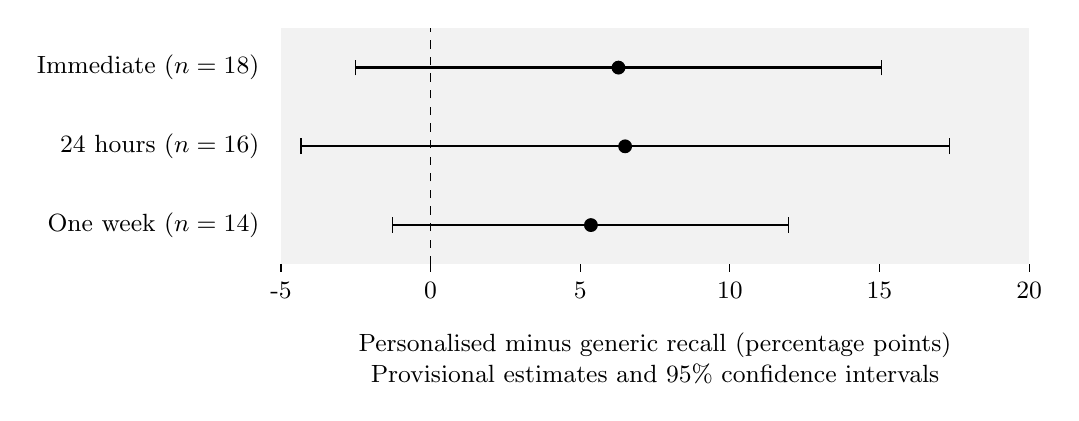
\begin{tikzpicture}[x=0.38cm,y=1cm]
\fill[gray!10] (-5,-0.5) rectangle (20,2.5);
\draw[dashed] (0,-0.5)--(0,2.5);
\foreach \x in {-5,0,5,10,15,20}{
  \draw (\x,-0.5)--(\x,-0.6) node[below,font=\small] {\x};
}
\draw[thick] (-2.5074,2)--(15.0630,2);
\draw (-2.5074,1.9)--(-2.5074,2.1);
\draw (15.0630,1.9)--(15.0630,2.1);
\fill (6.2778,2) circle (2.5pt);
\draw[thick] (-4.3317,1)--(17.3317,1);
\draw (-4.3317,0.9)--(-4.3317,1.1);
\draw (17.3317,0.9)--(17.3317,1.1);
\fill (6.5,1) circle (2.5pt);
\draw[thick] (-1.2595,0)--(11.9738,0);
\draw (-1.2595,-0.1)--(-1.2595,0.1);
\draw (11.9738,-0.1)--(11.9738,0.1);
\fill (5.3571,0) circle (2.5pt);
\node[anchor=east,font=\small] at (-5.4,2) {Immediate ($n=18$)};
\node[anchor=east,font=\small] at (-5.4,1) {24 hours ($n=16$)};
\node[anchor=east,font=\small] at (-5.4,0) {One week ($n=14$)};
\node[font=\small,align=center,anchor=north] at (7.5,-1.25) {Personalised minus generic recall (percentage points)\\Provisional estimates and 95\% confidence intervals};
\end{tikzpicture}
\caption{Paired recall differences in the frozen snapshot. Every interval crosses zero. The workbook remains blocked for interpretation pending data review.}
\label{fig:recallci}
\end{figure}

\section{Recall Quantity, Order, and Retention}
Immediate raw recall quantity averages 17.28 words in the generic condition and 18.89 in the personalised condition, giving a paired difference of 1.61 words. These means pool 20- and 25-target lists. It would therefore be incorrect to divide the overall word-count mean by 25 and expect it to reproduce the mean of trial-level accuracy.

The mean LCS proportion is 0.681 for the generic condition and 0.735 for the personalised condition at immediate recall. The paired difference is 0.054, with a 95\% interval from $-0.034$ to 0.143 and an unadjusted $p=.210$. The direction resembles the accuracy comparison, but the interval remains broad.

Kendall recalled-order means are 0.870 and 0.887 at immediate recall. At the nominal one-week follow-up, they are 0.872 and 0.708, using 13 complete pairs. This contrast illustrates why quantity and order should not be collapsed into a single claim. More recalled items do not necessarily mean better ordering among those items, and the set of recallable items changes over time.

For the 16 complete 24-hour retention pairs, mean accuracy change from immediate recall is $-0.145$ in the generic condition and $-0.159$ in the personalised condition. The paired difference in change is $-0.014$, with a 95\% interval from $-0.098$ to 0.069. The corresponding one-week changes are $-0.254$ and $-0.245$ for 14 pairs. These are within-participant retention calculations from the workbook. They are not obtained by subtracting the rows of Table~\ref{tab:recallmeans}, whose participant subsets differ.

The snapshot therefore does not support a claim that personalisation slows forgetting. Numerically higher delayed accuracy can arise alongside similar losses from immediate recall. A final retention analysis should preserve the same participants, target lists, and scoring rules across the compared timepoints.

\section{Questionnaire Outcomes}
Table~\ref{tab:questionnaires} reports condition means for the main questionnaire subscales. Scores are on the workbook's seven-point scale. The signs of the differences must be interpreted according to the construct: more enjoyment and more extraneous load are not favourable in the same way.

\begin{table}[htbp]
\centering
\small
\caption{Provisional questionnaire results. G denotes generic and P personalised; $\Delta=P-G$. Confidence intervals and $p$ values concern paired differences and are unadjusted.}
\label{tab:questionnaires}
\begin{tabular}{@{}lrrrrlr@{}}
\toprule
Measure & $n$ & G & P & $\Delta$ & 95\% CI & $p$ \\
\midrule
Interest/enjoyment & 17 & 5.85 & 6.02 & 0.17 & [$-0.18$, 0.52] & .326 \\
Perceived competence & 17 & 4.46 & 4.77 & 0.31 & [$-0.49$, 1.11] & .418 \\
Effort/importance & 17 & 5.58 & 5.39 & $-0.19$ & [$-0.52$, 0.15] & .252 \\
SUS presence & 14 & 5.17 & 5.48 & 0.31 & [$-0.03$, 0.65] & .069 \\
Intrinsic load & 18 & 4.61 & 4.19 & $-0.42$ & [$-1.34$, 0.51] & .356 \\
Germane load & 18 & 3.86 & 3.92 & 0.06 & [$-0.60$, 0.72] & .861 \\
Extraneous load & 18 & 3.13 & 2.69 & $-0.44$ & [$-1.04$, 0.15] & .134 \\
\bottomrule
\end{tabular}
\end{table}

Enjoyment is high in both conditions, with a small positive personalised-minus-generic difference. Perceived competence and presence are also numerically higher in the personalised condition. Intrinsic and extraneous load are numerically lower. However, every confidence interval shown includes zero, and the duplicate-record issues directly concern questionnaire data.

The presence result should not be described as significant or nearly proven because its unadjusted $p$ value is .069. It is one of several outcomes, uses only 14 pairs, and remains subject to source reconciliation. Nor does it establish a mechanism by which personalisation improves recall. Such a claim would require an appropriate analysis of the relationship between presence and recall, as well as stronger control over alternative explanations.

Effort/importance is slightly lower in the personalised condition. Lower effort can indicate easier use, less engagement, or a different interpretation of the activity. The questionnaire alone does not determine which explanation applies. Similarly, the small difference in germane load does not show that the quality of learning was unchanged.

The separate three-item germane score is retained as exploratory in the workbook. It is not substituted for the two-item main score in Table~\ref{tab:questionnaires}. Legacy IPQ outcomes are not combined with SUS presence because the instruments and scoring issues differ.

\section{Recall Time}
For the 14 timed immediate-recall pairs, mean recall duration is 218.35 seconds in the generic condition and 259.69 seconds in the personalised condition. The mean difference is 41.34 seconds, with a 95\% interval from $-3.43$ to 86.10 seconds and an unadjusted $p=.067$.

This does not show that the personalised palace is less efficient. Participants may spend longer because they recover more words or continue searching for additional items. Conversely, a long duration could reflect difficulty retrieving the route. The five-minute limit in the revised protocol also needs to be checked against the timing conventions and individual records. No delayed-duration comparison is reported because the workbook contains no complete timed pairs at those follow-ups.

\section{Discussion}
\subsection{What the Current Comparison Can Say}
The numerical pattern is compatible with a possible advantage for the personalised workflow, but it does not establish one. The immediate mean difference is positive, yet the participant-level directions are mixed and the confidence interval crosses zero. At later timepoints, differences remain uncertain and participant coverage decreases.

The findings should not be described as contradicting studies of VR immersion or active spatial binding. Those studies changed different aspects of the task~\cite{krokos2019,reggente2020}. A system may benefit from active placement in both conditions while showing a smaller additional difference between a generic and a familiar palace. The present study is concerned with that additional difference.

\subsection{Familiarity, Construction, and Exposure}
The personalised condition combines several experiences. Participants bring prior knowledge of their home, actively edit the virtual environment, and spend additional time working with it. Any eventual difference between conditions could reflect one or more of those factors.

The familiar-layout rationale is supported by research on object and spatial memory~\cite{merriman2016}, but this does not identify familiarity as the cause of the present numerical pattern. A stronger follow-up design could compare a generic palace, a familiar palace prepared for the participant, and an unfamiliar palace that the participant edits. Exposure time would also need to be measured or controlled.

\subsection{Mixed Materials and Ceiling Effects}
Pilot development aimed to avoid a task that participants could complete perfectly in both conditions. Nevertheless, the current snapshot contains both earlier and harder lists. Pooling them may combine different levels of task difficulty and different opportunities for improvement.

Normalised accuracy addresses the arithmetic difference between 20 and 25 targets, but does not remove differences in the words or their mnemonic images. The final analysis should therefore report results for the intended main-study materials and examine sensitivity to the inclusion of earlier sessions. Any version-based subgroup analysis will be exploratory unless its role was specified before examining outcomes.

\subsection{Missingness and Order}
The decrease from 18 immediate pairs to 16 at 24 hours and 14 at one week changes the sample being described. The missing participants may differ in motivation, availability, or memory performance. This draft does not assume that follow-up data are missing at random.

Order is another unresolved issue. The workbook's session-order diagnostic contains no complete pairs, despite planned counterbalancing. That is not evidence that there was no order effect; it means the necessary diagnostic is currently unavailable. Recovering actual order from session records is required before practice and fatigue can be assessed.

\subsection{Practical Value and Remaining Evidence}
A personalised palace may be useful even if its mean recall advantage is modest, for example if users prefer to return to it over time. Conversely, a short-term recall gain may not justify a long creation stage. The current dataset cannot settle that trade-off without verified preparation-time, repeated-use, and preference evidence.

The system contribution is therefore distinct from the efficacy claim. The documented workflow shows how a familiar environment can be prepared, edited, and used for cue placement. Whether that workflow improves recall enough to justify its costs remains an empirical question. Final conclusions should follow the reconciled records, including the possibility of an inconclusive or small difference.

